% \documentclass[article]{standalone}
\documentclass[tikz]{standalone}

\usepackage{hyperref}
%\usepackage{hyperref, tikz}

% Determine flow chart stuff
\usetikzlibrary{shapes.geometric, arrows} % Arrows library
% Define block styles
%\tikzstyle{decision} = [diamond, draw, fill=blue!20, text width=4.5em, text badly centered, node distance=3cm, inner sep=0pt]
\tikzstyle{bblock} = [rectangle, draw, fill=blue!20, text width=11em, text centered, rounded corners, minimum height=4em, node distance = 7em]
\tikzstyle{yblock} = [rectangle, draw, fill=yellow!20, text width=11em, text centered, rounded corners, minimum height=4em, node distance = 7em]
\tikzstyle{rblock} = [rectangle, draw, fill=red!20, text width=11em, text centered, rounded corners, minimum height=4em, node distance = 7em]
\tikzstyle{wblock} = [rectangle, draw, fill=white, text width=11em, text centered, rounded corners, minimum height=4em, node distance = 7em]
\tikzstyle{secret} = [text width=1em, text centered, rounded corners, minimum height=1em, node distance = 2em]
\tikzstyle{line} = [draw, very thick, color=black, -latex']
\tikzstyle{rcloud} = [draw, ellipse, fill=red!20, text width=10em, node distance=5cm, minimum height=4em]
\tikzstyle{wcloud} = [draw, ellipse, fill=white, text width=10em, node distance=5cm, minimum height=4em]

%Change to sans serif font
\renewcommand{\familydefault}{\sfdefault}		%Alone with use Computer Modern sans serif
\usepackage{sansmathfonts}

\hypersetup{
    linktoc=all,     %set to all if you want both sections and subsections linked
}

\begin{document}

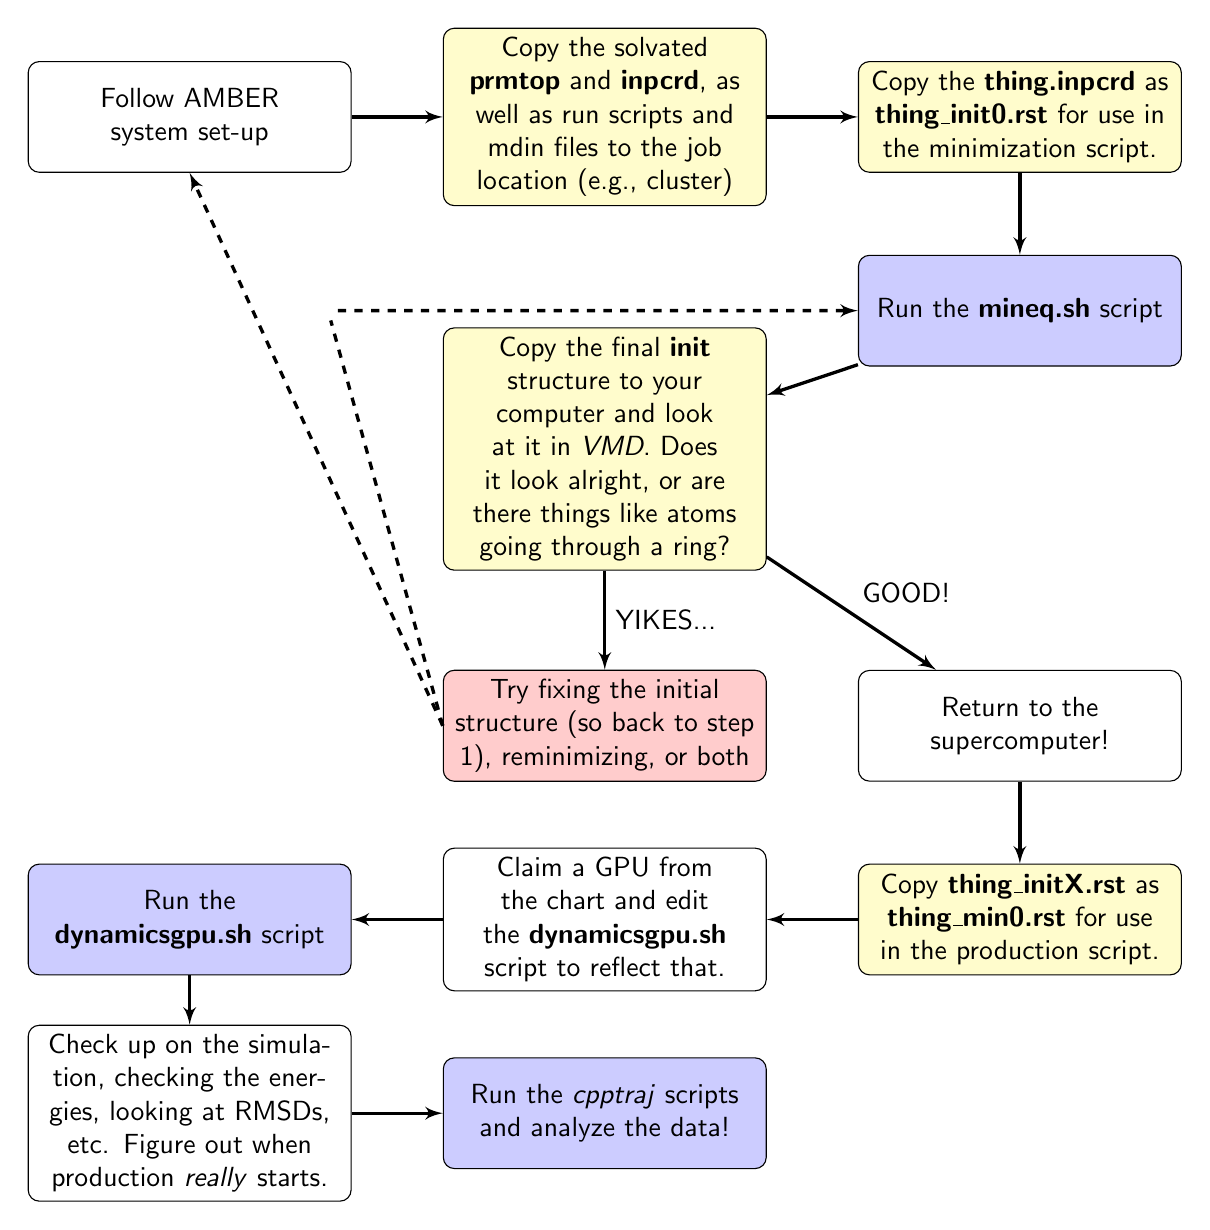
\begin{tikzpicture}[node distance = 0.5cm, auto, align=flush left]
    % Place nodes
%    \node [wblock] (setup) {\hyperref[https://emleddin.github.io/comp-chem-website/AMBERguide-systems-overview.html]{Follow AMBER system set-up}};
    \node [wblock] (setup) {Follow AMBER system set-up};
    \node [yblock, right of=setup, node distance=15em] (copy) {Copy the solvated \textbf{prmtop} and \textbf{inpcrd}, as well as run scripts and mdin files to the job location (e.g., cluster)};
    \node [yblock, right of=copy, node distance=15em] (rename1) {Copy the \textbf{thing.inpcrd} as \textbf{thing\_init0.rst} for use in the minimization script.};
    \node [bblock, below of=rename1] (min) {Run the \textbf{mineq.sh} script};
    \node [left of=min, node distance=25em] (ghost) {}; % I'm invisible
    \node [yblock, below of=copy, node distance=12em] (check) {Copy the final \textbf{init} structure to your computer and look at it in \emph{VMD}. Does it look alright, or are there things like atoms going through a ring?};
    \node [wblock, below of=min, node distance=15em] (continue) {Return to the \\ supercomputer!};
%    \node [rblock, left of=continue, node distance=15em] (fixit) {Try fixing the initial structure (so back to \hyperref[https://emleddin.github.io/comp-chem-website/AMBERguide-systems-overview.html]]{step 1}), reminimizing, or both};
    \node [rblock, left of=continue, node distance=15em] (fixit) {Try fixing the initial structure (so back to step 1), reminimizing, or both};
    \node [yblock, below of=continue] (rename2) {Copy \textbf{thing\_initX.rst} as \textbf{thing\_min0.rst} for use in the production script.};
    \node [wblock, left of=rename2, node distance=15em] (claimGPU) {Claim a GPU from the chart and edit the \textbf{dynamicsgpu.sh} script to reflect that.};
    \node [bblock, left of=claimGPU, node distance=15em] (prod) {Run the \\ \textbf{dynamicsgpu.sh} script};
    \node [wblock, below of=prod] (monitor) {Check up on the simulation, checking the energies, looking at RMSDs, etc. Figure out when production \emph{really} starts.};
    \node [bblock, right of=monitor, node distance=15em] (analyze) {Run the \emph{cpptraj} scripts and analyze the data!};
    % Draw edges
    \path [line] (setup.east) -- (copy);
    \path [line] (copy) -- (rename1);
    \path [line] (rename1) -- (min);
    \path [line] (min) -- (check);
    \path [line] (check) -- node {YIKES...} (fixit);
    \path [line,dashed] (fixit.west) -- (setup.south);
    \path [line,dashed] (fixit.west) -- (ghost) -- (min);
    \path [line] (check) -- node {GOOD!} (continue);
    \path [line] (continue) -- (rename2);
    \path [line] (rename2) -- (claimGPU);
    \path [line] (claimGPU) -- (prod);
    \path [line] (prod) -- (monitor);
    \path [line] (monitor) -- (analyze);
    %\path [line] (loops) -| node [near start] {yes} (update);
    %\path [line] (update) |- (identify);
    %\path [line] (decide) -- node {no}(stop);
    %\path [line,dashed] (expert) -- (init);
    %\path [line,dashed] (system) -- (init);
    %\path [line,dashed] (system) |- (evaluate);
\end{tikzpicture}

\end{document}
